\section{Cross section}\index{Cross Section}
Imagine a 2-D box in deep space, away from gravity, containing some number of large 2D disks.  If you threw a ball at the box, the probability of hitting a disks is related to the ratio of the cross sectional area of the box to the cross sectional area of the disks.  The cross sectional area of the disks is their �cross section� and it has units of area.  If you look at a solid and imagine scattering particles off the nuclei inside them, it is similar.  Remember that solids are, after all, mostly empty space.  If you project all the nuclei into the 2D front face of the solid, you have our 2-D box.  The cross section area of a nuclei is measured in fm2.  For low energy scattering by the strong force, since the strong force only has a very short range, and interactions can only happen if the ball virtually touches the nucleus, this is a good approximation.  A unit commonly used in the barn, which is 10-28 m2.  Nuclear �cross sections� are around 80 mbarns.  For forces with a longer range, such as E\&M, we define instead an �effective� area.  See any introductory book on particle physics for a more precise definition.

What if instead you threw a steady stream of balls at the box and wanted to calculate the rate at which balls hit beads and are deflected?  Also, as you can imagine, in realistic beams the projectiles do not march single file.  You should imagine them moving in a cylinder with some cross section, like:

If the number of balls in the beam per unit area is na, and the velocity of the balls is v,  then the number of balls reaching the target per second is

\[\Phi = n_{a}v\]

and \(\Phi\) is called the flux.  What are the units of \(\Phi\)?

The number of scatters per second is then

\[\frac{dN}{dt}=\Phi !I could not figure out how to this simble here here!\]

(check that the units work).

Now, you may ask what happens in a collider?  Well, it is just the same.  You can always move to a frame where one of the protons is at rest, do the calculation there, and move back.  We will see in the next section why our calculation of the cross section does not depend on the frame in which it is calculated.

\section{s, t, u, and q squared}\index{s, t, u, and q squared}

As we have seen, in relativity, there are �invariants� that will be measured to be the same by all observers, regardless of their frame and relative motion of the particle.  One of these is the length of a particle�s 4-momentum, which is its mass.  In collisions, there are a few of these variables that are important, as cross sections calculated from the standard model must be functions only of these variables and numeric factors.  The most important ones were unimaginable given the names s, t, u and Q2.  Imagine some kind of reaction (could be photon exchange, gluon exchanged, Z exchange etc) where two particles a and b come in and two particles c and d come out  (called a 2 to 2 reaction).

\begin{figure}[h]
\centering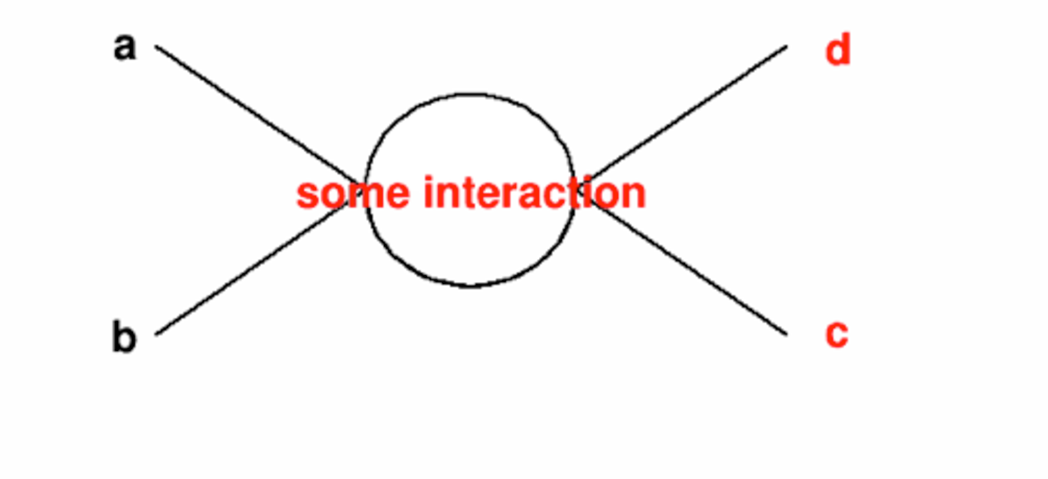
\includegraphics[scale=0.5]{./protonprotoncollisions/Pictures/fig1.pdf}
\caption{generic interaction of 2 particles going to 2 particles}
\label{fig:fig1}
\end{figure}

If \(p_{a}\) is the 4-momentum of particle A and the 4-momenta of the other particles are named similarly, then

\[s=(p_{a}+p_{b})^{2}\]
\[t=(p_{a}-p_{c})^{2}\]
\[u=(p_{a}-p_{d})^{2}\]

Remember: the square here means dot product, and the dot product of a 4-vector is the square root of the product of the first components (time-like components) minus the dot product of the 3D part of the 4 vector.  So s, t, u are a bit like a mass.  All these variables have units of \(GeV^{2}\).

Another important variable is \(Q^{2}\).  This can be u for some interactions and s for others.  It is the �mass� of the virtual particle that is exchanged in the interaction (the photon, W, Z etc).  Now, you may say: but the photon is massless!  But, that is only if it is observable.  The photon can be �offshell� as long as it is unobservable, meaning that it has a non-zero mass.  You will learn more about this when you study quantum mechanics.

It can be shown in quantum field theory that, in the frame where the 4-momentum of particles a and b are equal but opposite and have high enough energy that we can neglect their mass, that the cross section can be calculated from the physics of the standard model using a simple formula

\[
\frac{d?}{d\Omega} = \frac{1}{64\Pi^{2}s}\frac{P_{f}}{P_{i}}|M|^{2}
\]

where \(p_{f}\) is the magnitude of the 3-momenta of either particle c or d (why doesn�t it matter which?) and pi is that of either a or b.  What will the ratio of pf to pi be if particles c and d both have momenta large compared to their mass as well?

\(|M|^{2}\)  is a factor called the �matrix element� which is calculated from the standard model and must be a function of s, t, u and numeric factors.

\section{What is in a Proton}\index{What is in a Proton}
You may have been taught that a proton contains two up quarks and a down quark.  This is not true.  In fact, only half the momentum of a proton is carried by quarks.  What carries the other half?  This is a complicated question.  Roughly, we can say that about half the momentum is carried by the up and down quarks, and about half by gluons.  One of the goals of nuclear physics is to understand how the momentum distribution of the proton is divided amoung the protons constituents.  The �Parton Distribution Functions� or PDFs give the probability of finding a �parton� (a constituent of the proton, like a quark or gluon) with a fraction of the proton momentum x.  When you sum over all partons and all x, you should get 1 (when you add them all together, you have the whole momentum of the proton).  The figure below shows results from measurements.

\begin{figure}[h]
\centering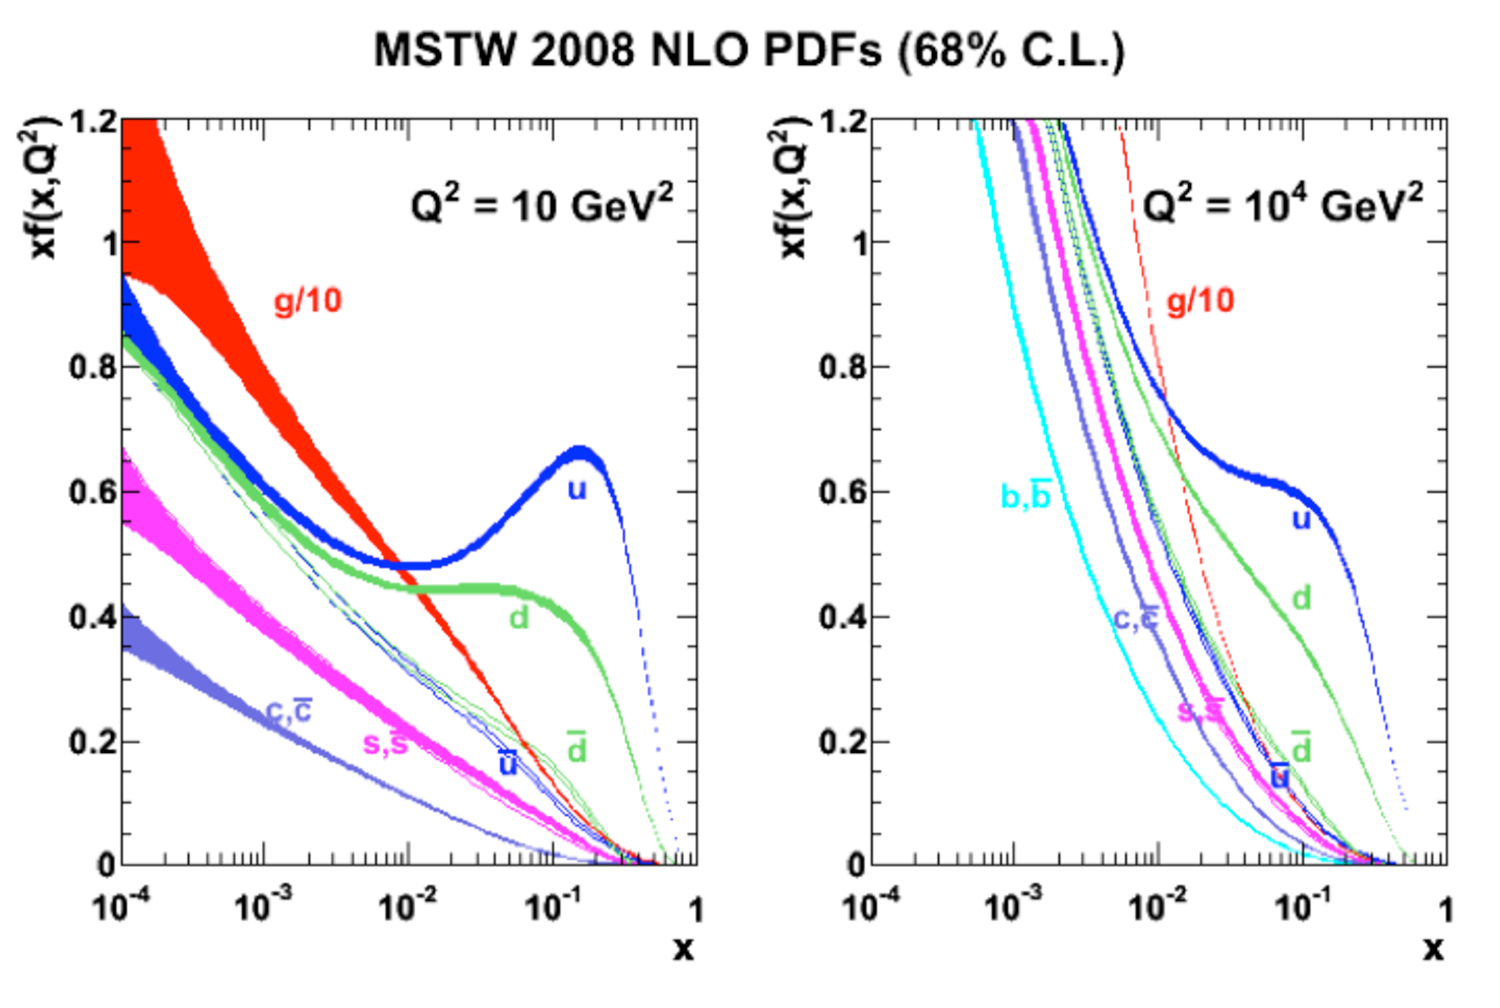
\includegraphics[scale=0.5]{./protonprotoncollisions/Pictures/fig2.pdf}
\caption{probability of finding a parton that has a fraction x of the proton momentum times x for different parton flavors}
\label{fig:fig2}
\end{figure}
However, the truth is, if you look inside a proton, what you see depends on how closely you look. The closer you look, the more detail you see.  Interactions with large \(Q^{2}\) look more closely that those that don�t (think about the uncertainty principal and it may help you understand).  That is why there are two figures in the picture shown above.  One shows what the proton looks like if you probe it with a virtual particle with low \(Q^{2}\) and the other shows it with a higher \(Q^{2}\) probe.

How do we do this?  Most of the information comes from �fixed target experiements�, which collide a beam of particles with some kind of target, perhaps copper or something else that won�t melt in a high radiation environment, and from the �HERA� collider in Hamburg Germany, which collides electrons with protons.

magine two possible beams in a fixed target experiment: muons and neutrinos.  Muons will interact with the up and down quarks (and other quarks) in the  proton via photons, more with the up quarks than with the down quarks due to their larger electric charge.  If we switch to a different target which has a different ratio of neutrons to protons, we get a different ratio of up and down quarks and different scattering rates.  Neutrinos interact with the protons and neutrons via the weak force, mostly the Z boson.  These also interact differently with up and down quarks, but in a different way.  Groups of theorists, such as �MRST� and �CTEQ� take all this data and untangle from it the �parton distribution functions�.  Note that neither type of beam interacts directly with gluons and therefore there is larger uncertainty on this part of the PDF than that of the quarks.

\section{Calculation of a cross section in proton proton collisions}\index{Calculation of a cross section in proton proton collisions}

In a proton-proton collision, the particles and b are partons in the proton.  For a given final state (particles c and d), there can be a variety of different initial states that can occur.  For example, a Z boson can be created when an up quark annihilates with an anti-up quark or it can be created when an down quark annihilates with an anti-down quark.  It is like our bean has different kinds of balls that have a different effective cross section to interact with the target.  How can we calculate the total cross section for any two partons in the proton to go to a Z and then into, say an electron-positron pair?  We need to integrate over all possible initial states:

\[!!!!I don't even no what to look up to add this math!!!!\]

where the q�s represent the PDFs for the quarks.

\section{What happens when two protons collide?}\index{What happens when two protons collide?}
First remember that quantum mechanics applies.  We can calculate the probability of certain kinds of interactions, but we can not predict event by event which one will occur.  The pie chart below shows the fraction of collisions that result in different types of interactions.

\begin{figure}[h]
\centering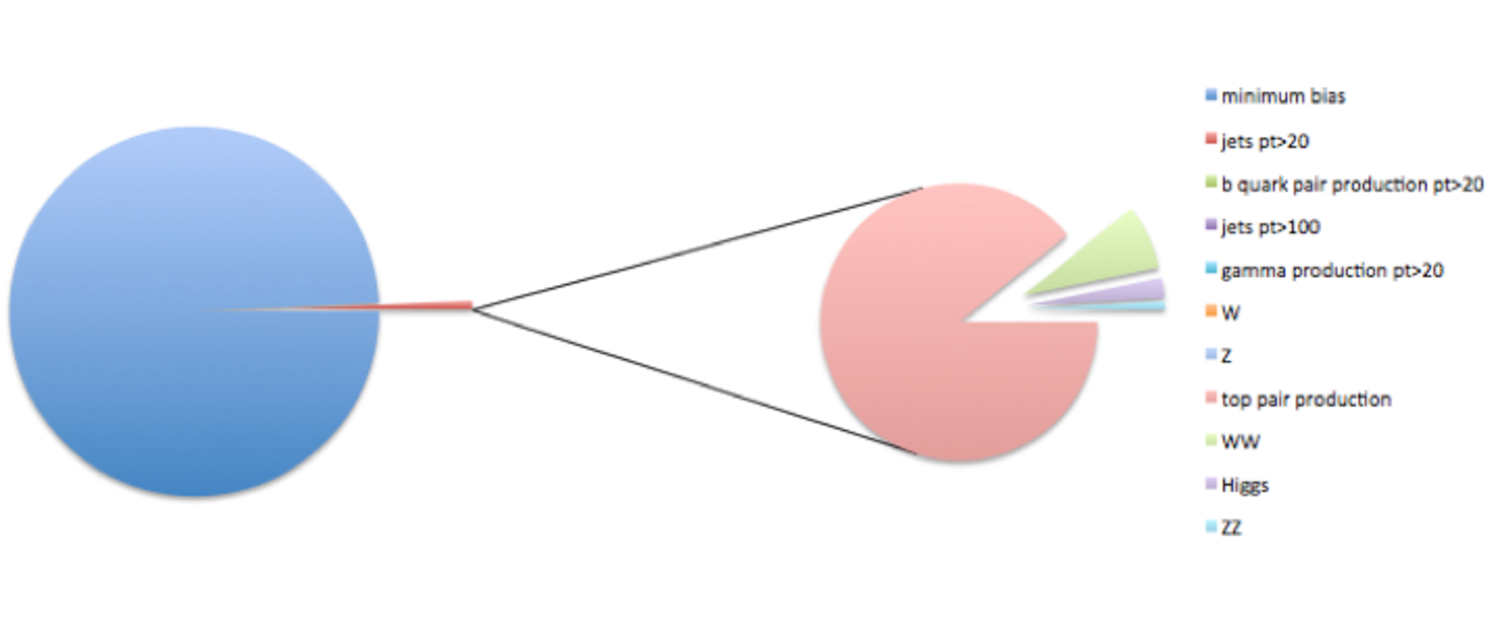
\includegraphics[scale=0.5]{./protonprotoncollisions/Pictures/fig3.pdf}
\caption{Pie chart showing relative probabilities of different types of interactions in proton-proton collisions}
\label{fig:fig3}
\end{figure}
Another way to look at this is for the cross

\begin{figure}[h]
\centering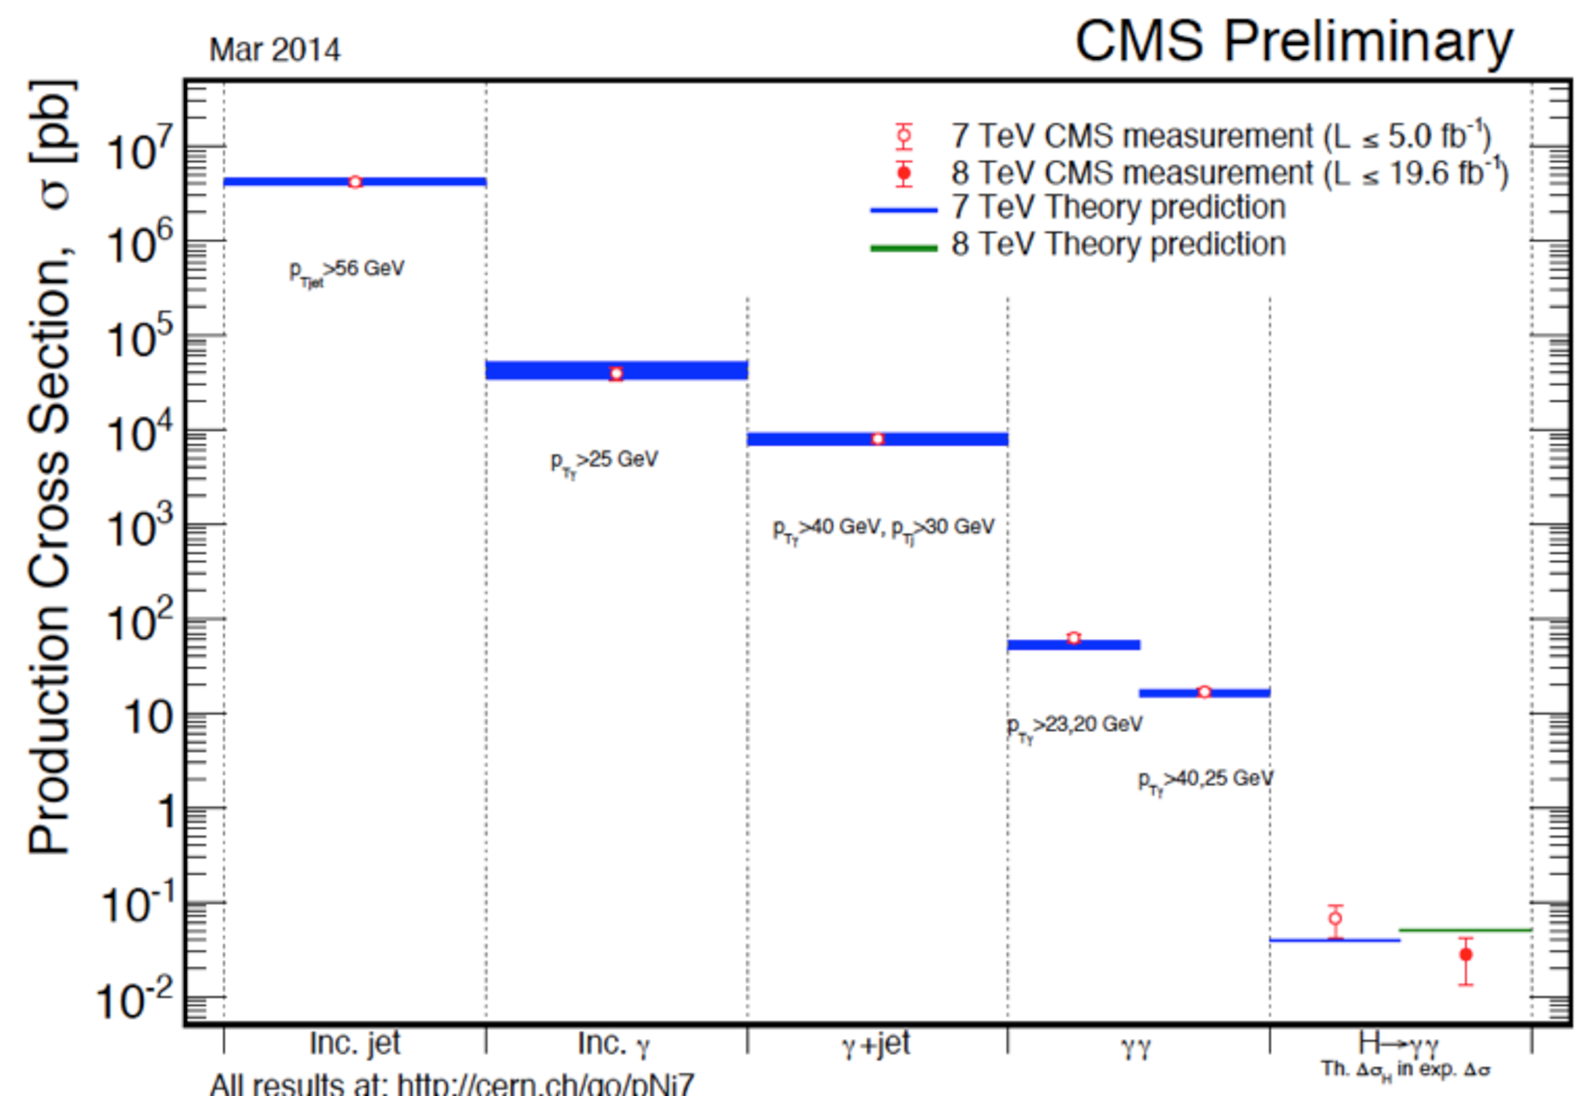
\includegraphics[scale=0.5]{./protonprotoncollisions/Pictures/fig4.pdf}
\caption{!!! No Caption In Word Doc !!!}
\label{fig:fig4}
\end{figure}
\begin{figure}[h]
\centering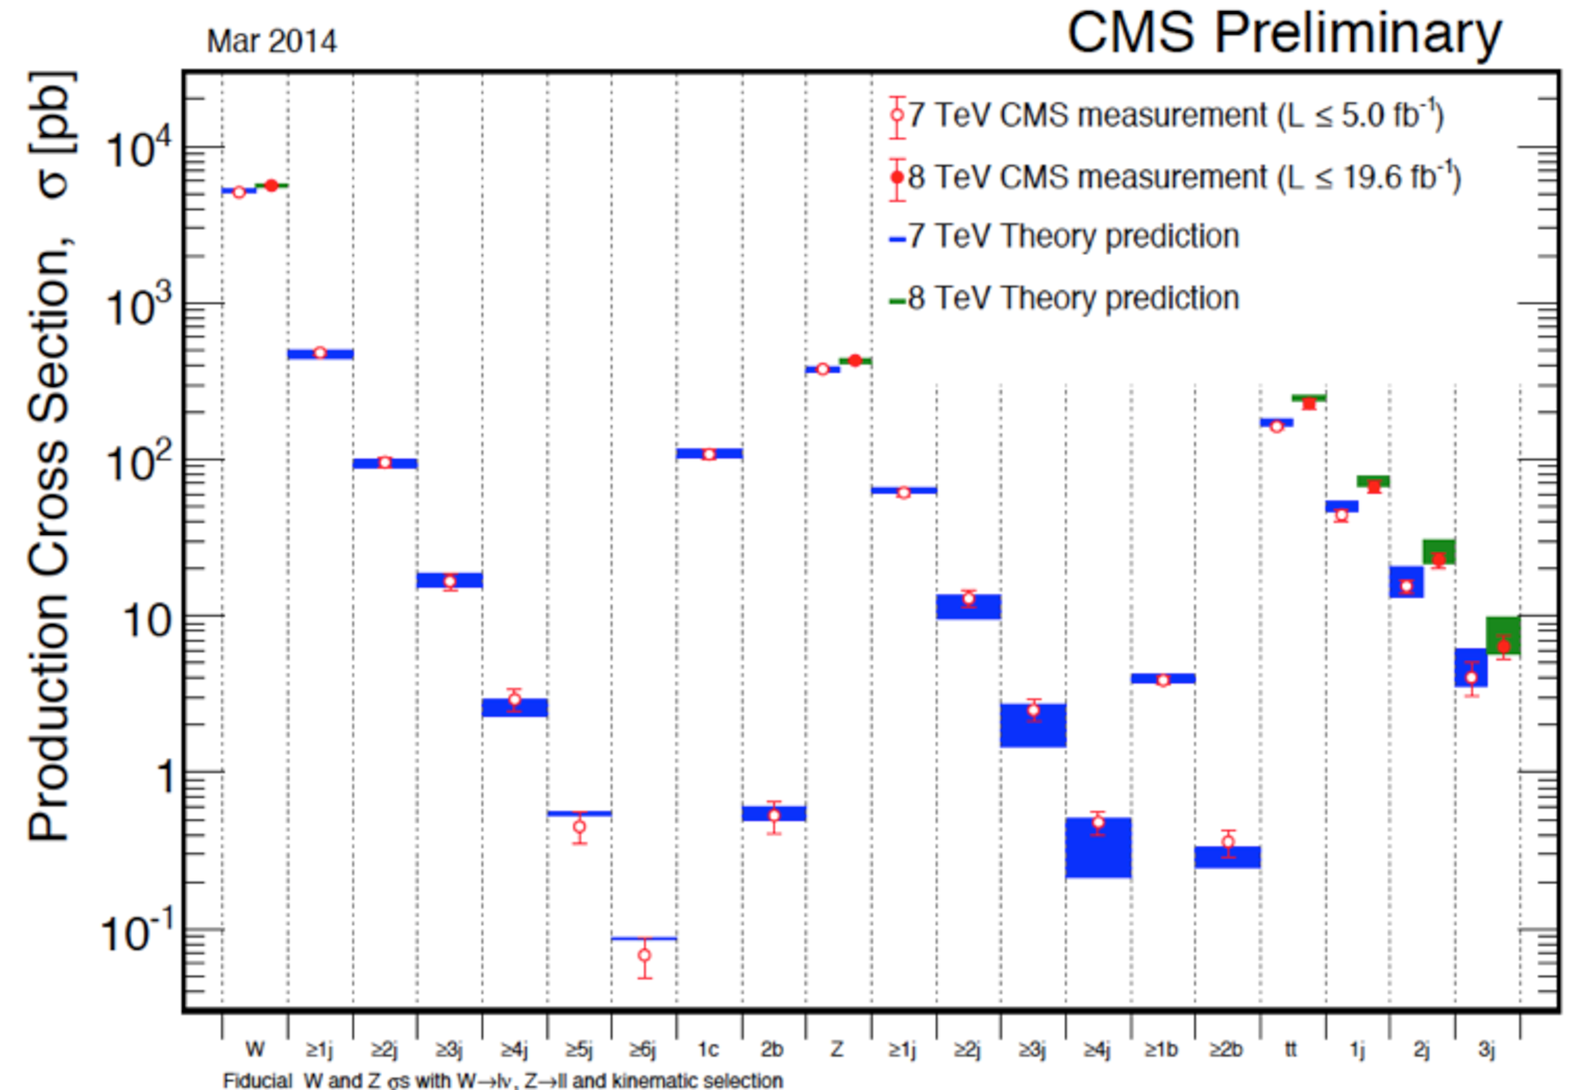
\includegraphics[scale=0.5]{./protonprotoncollisions/Pictures/fig5.pdf}
\caption{!!! No Caption In Word Doc !!!}
\label{fig:fig5}
\end{figure}


What are these things?

\section{Minimum bias interaction}\index{Minimum bias interaction}

The most common thing to occur is that a small amount of momentum is exchanged between the proton, in the form of gluons, or color-neutral combinations of gluons, resulting in a few pions being spit out.  A cartoon might look like:

\begin{figure}[h]
\centering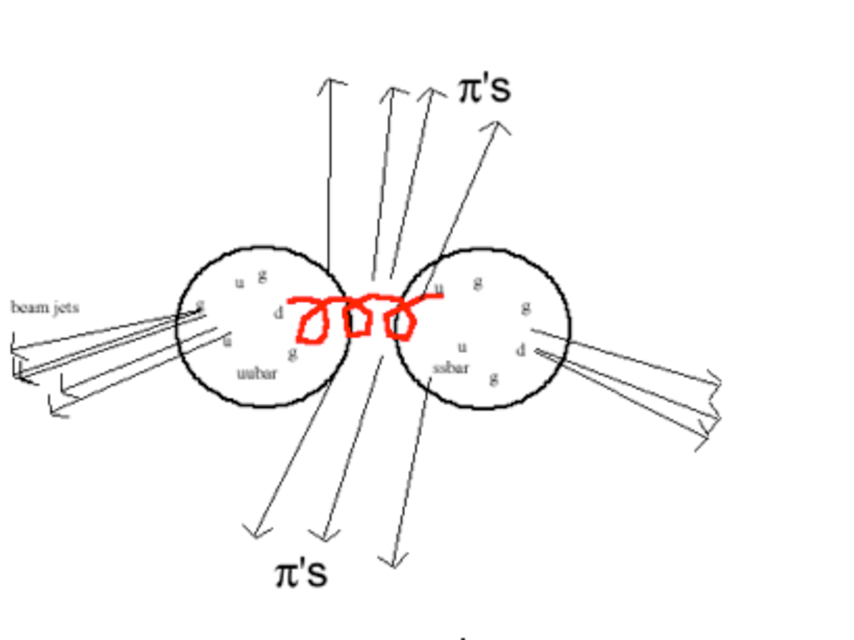
\includegraphics[scale=0.5]{./protonprotoncollisions/Pictures/fig6.pdf}
\caption{carton of a minimum bias interaction}
\label{fig:fig6}
\end{figure}

\section{Jets}\index{Jets}

\begin{figure}[h]
\centering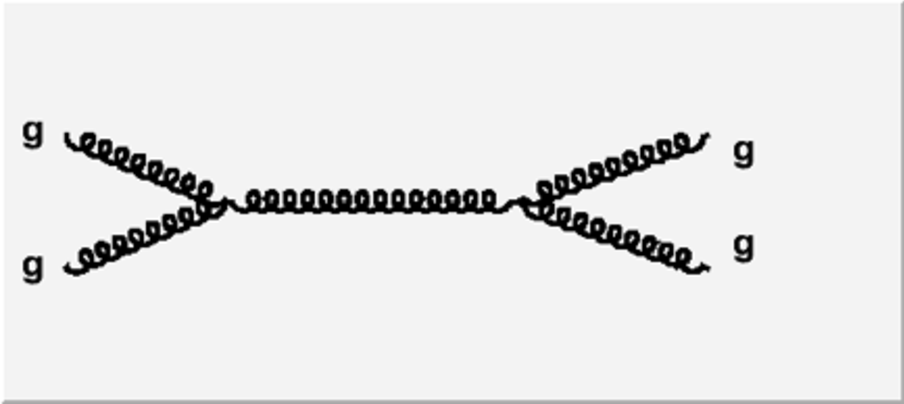
\includegraphics[scale=0.5]{./protonprotoncollisions/Pictures/fig7.pdf}
\caption{!!!NO CAPTION!!!}
\label{fig:fig7}
\end{figure}

\begin{figure}[h]
\centering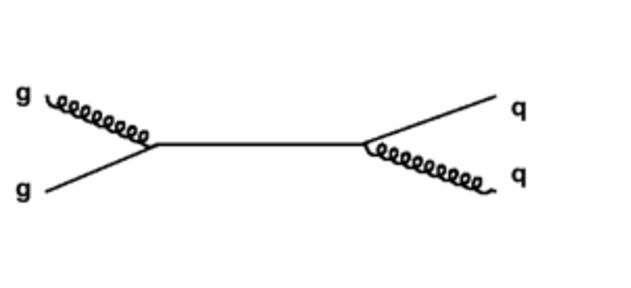
\includegraphics[scale=0.5]{./protonprotoncollisions/Pictures/fig8.pdf}
\caption{!!!NO CAPTION!!!}
\label{fig:fig8}
\end{figure}

\begin{figure}[h]
\centering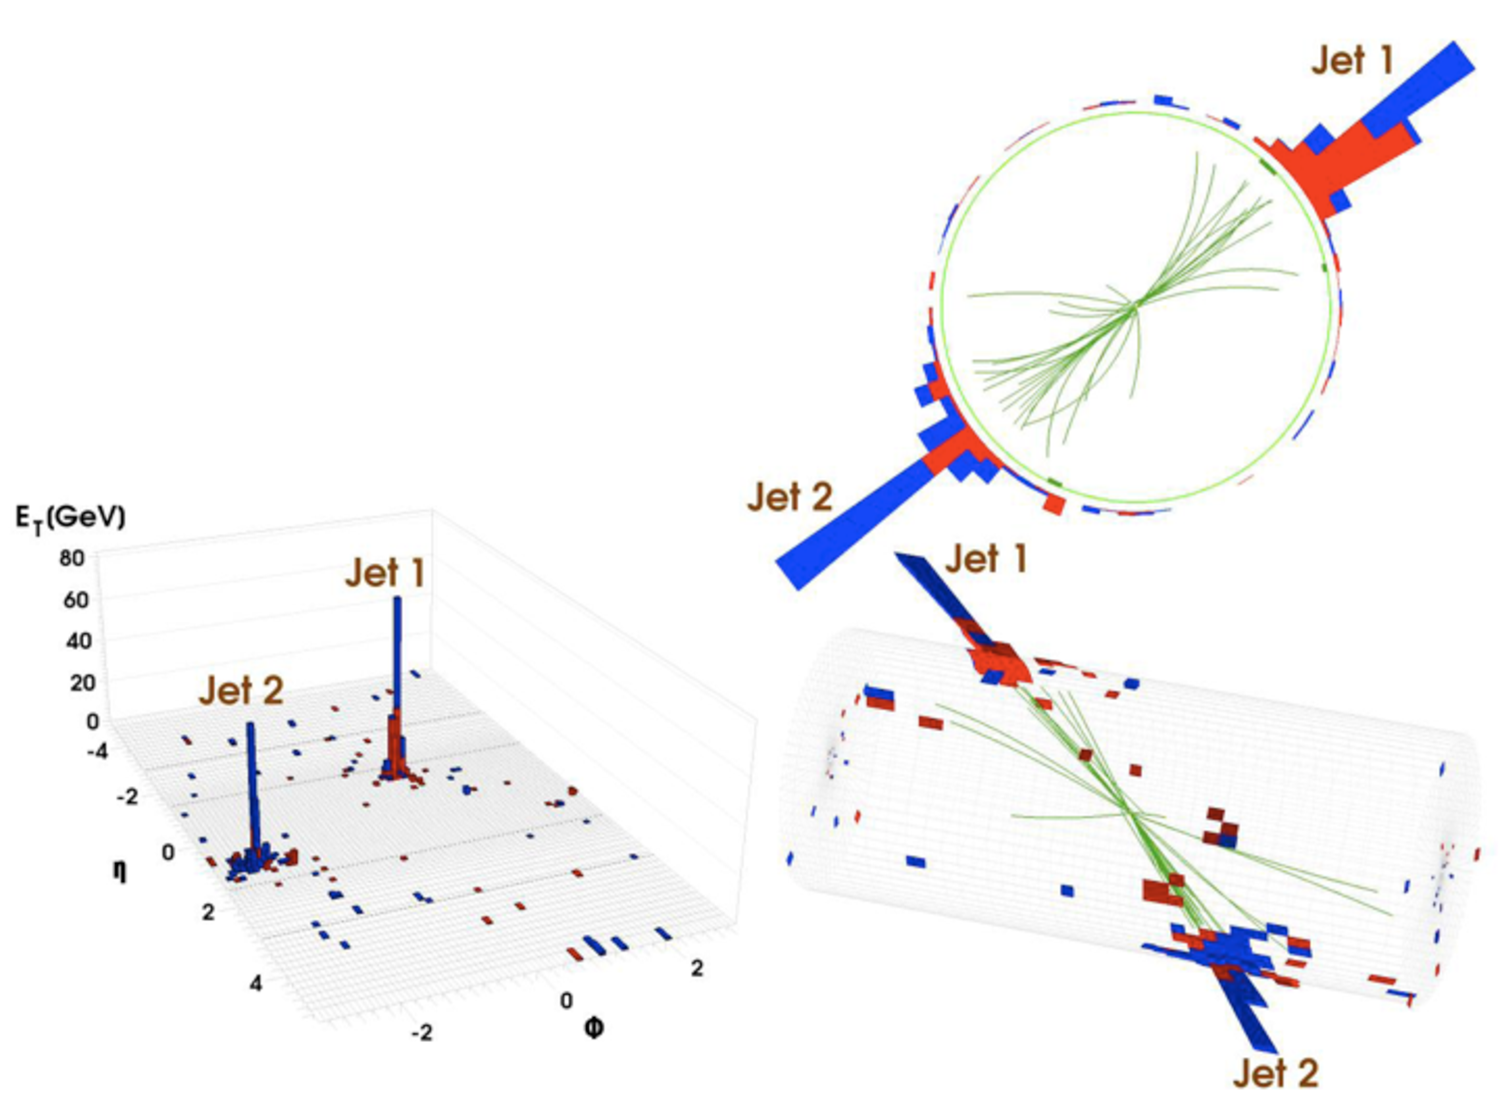
\includegraphics[scale=0.5]{./protonprotoncollisions/Pictures/fig9.pdf}
\caption{!!!NO CAPTION!!!}
\label{fig:fig9}
\end{figure}

\begin{figure}[h]
\centering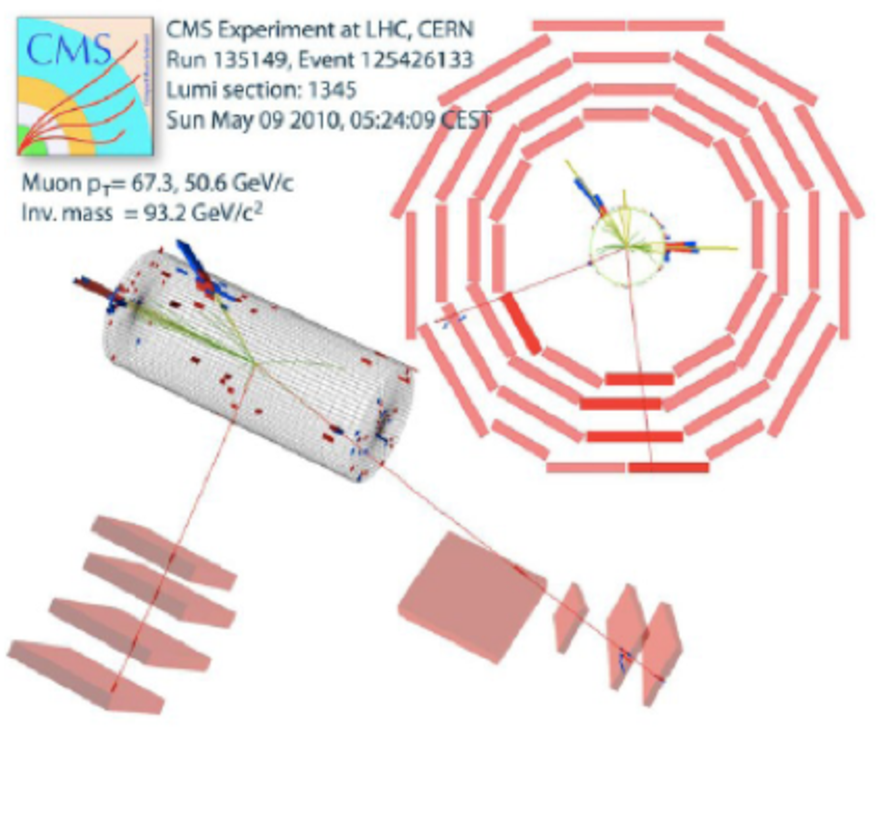
\includegraphics[scale=0.5]{./protonprotoncollisions/Pictures/fig10.pdf}
\caption{!!!NO CAPTION!!!}
\label{fig:fig10}
\end{figure}

\begin{figure}[h]
\centering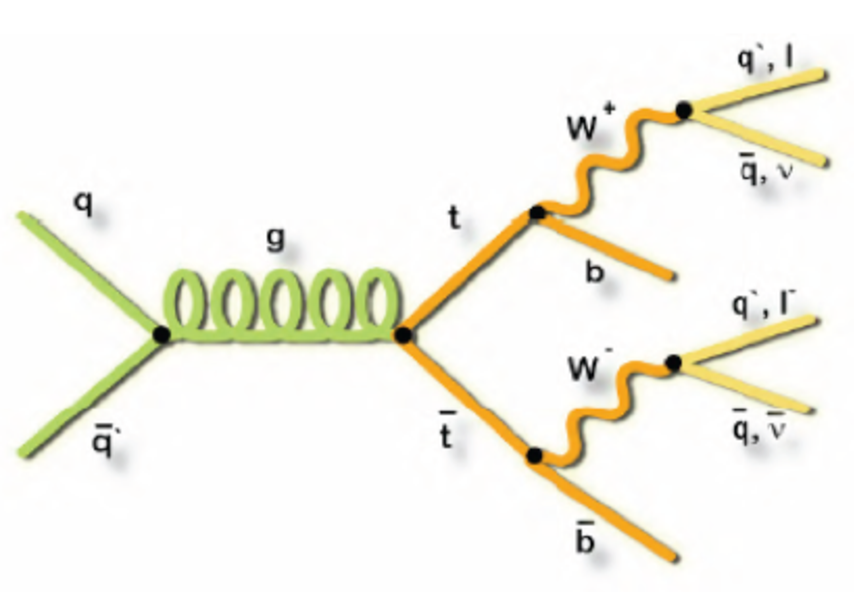
\includegraphics[scale=0.5]{./protonprotoncollisions/Pictures/fig11.pdf}
\caption{!!!NO CAPTION!!!}
\label{fig:fig11}
\end{figure}

\begin{figure}[h]
\centering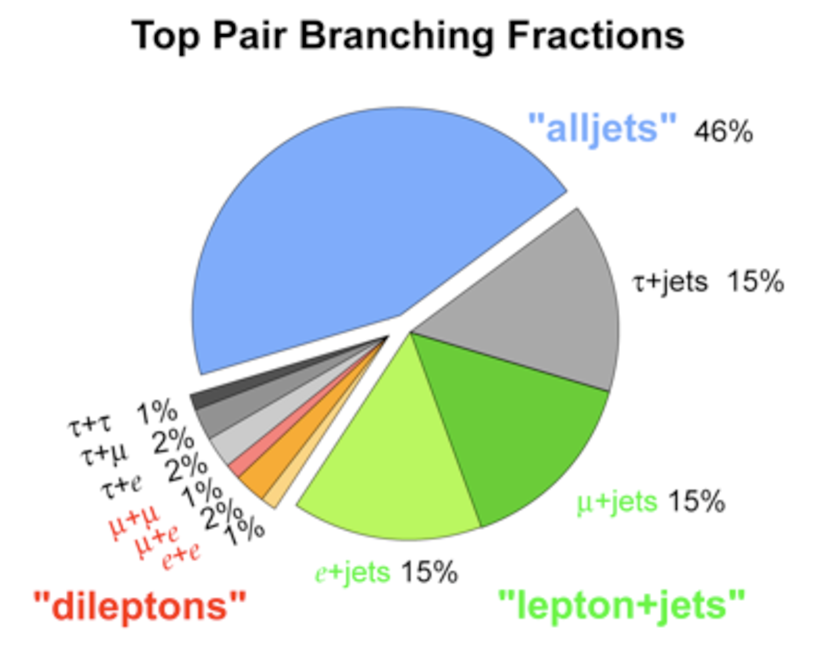
\includegraphics[scale=0.5]{./protonprotoncollisions/Pictures/fig12.pdf}
\caption{!!!NO CAPTION!!!}
\label{fig:fig12}
\end{figure}

\begin{figure}[h]
\centering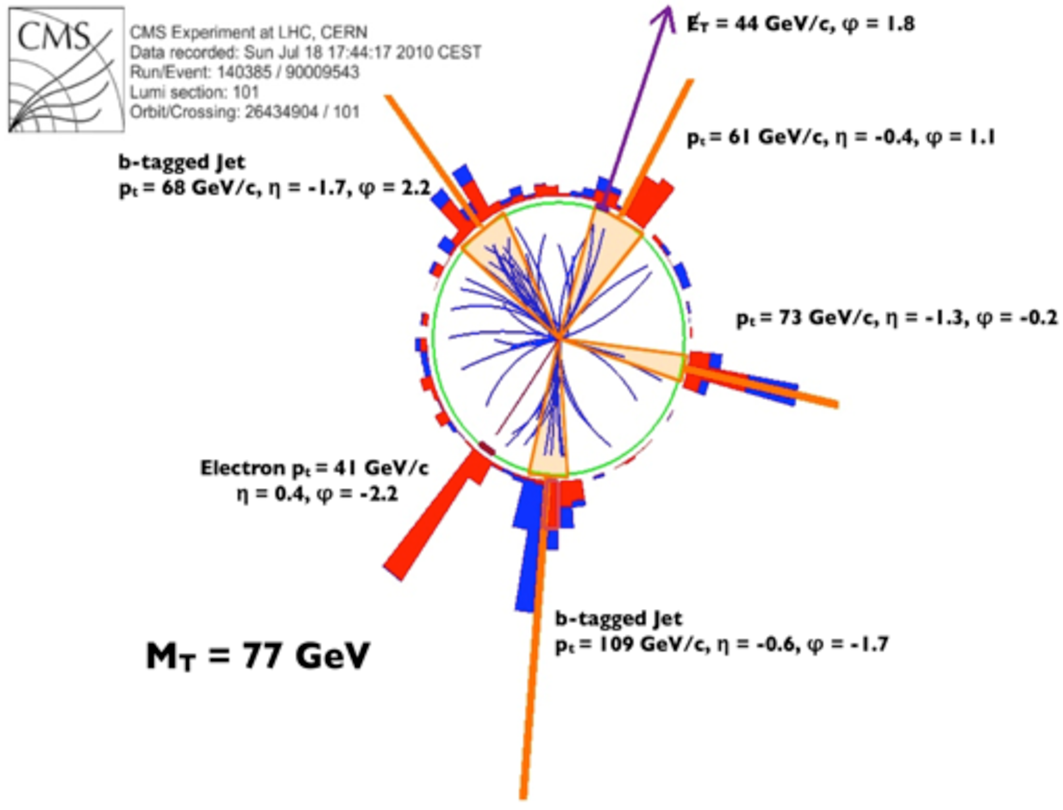
\includegraphics[scale=0.5]{./protonprotoncollisions/Pictures/fig13.pdf}
\caption{!!!NO CAPTION!!!}
\label{fig:fig13}
\end{figure}

\section{Further Reading}\index{Further Reading}

\begin{itemize}
\item http://xxx.lanl.gov/abs/hep-ph/9606399
\item http://iopscience.iop.org/0034-4885/70/1/R02/
\item �Modern Particle Physics� by Mark Thomson
\item �Introduction to Elementary Particle Physics� by Alessandro Bettini
\end{itemize}
